% !TEX root = ./article.tex

\documentclass{article}

\usepackage{mystyle}
\usepackage{myvars}



%-----------------------------

\begin{document}

	\maketitle % Insert title

	\thispagestyle{fancy} % All pages have headers and footers


%-----------------------------
%	ABSTRACT
%-----------------------------

	\begin{abstract}
		\noindent [TODO ]
	\end{abstract}

%-----------------------------
%	TEXT
%-----------------------------


	\section{Introducción}
	\label{sec:introducción}

		\paragraph{}
		[TODO]

		\subsection{$K$-vecinos más cercanos}

			\paragraph{}
			[TODO]

	\section{La figura \ref{e1:plot} muestra un conjunto de entrenamiento con ejemplos positivos (estrellas) y negativos (círculos). Se desea clasificar la nueva instancia $<3,3>$ mediante el algoritmo $K$-vecinos más próximos. Obtener la clasificación para los valores de $K=\{ 1, 3, 5\}$ utilizando las distancias indicadas a continuación}
	\label{sec:e1}

		\paragraph{}
		En este ejercicio se realiza una clasificación mediante el algoritmos de clasificación basado en instancias \emph{K-NN}. El conjunto de datos está compuesto por $7$ instancias caracterizadas por $2$ atributos númericos de caracter entero y la clase de destino de tipo binario (\emph{ESTRELLAS} o \emph{CIRCULOS}). Puesto que el espacio del conjunto de datos está formado por dos dimensiones este se puede representar de forma gráfica tal y como se muestra en la figura \ref{e1:plot}.

		\begin{figure}
			\begin{center}
				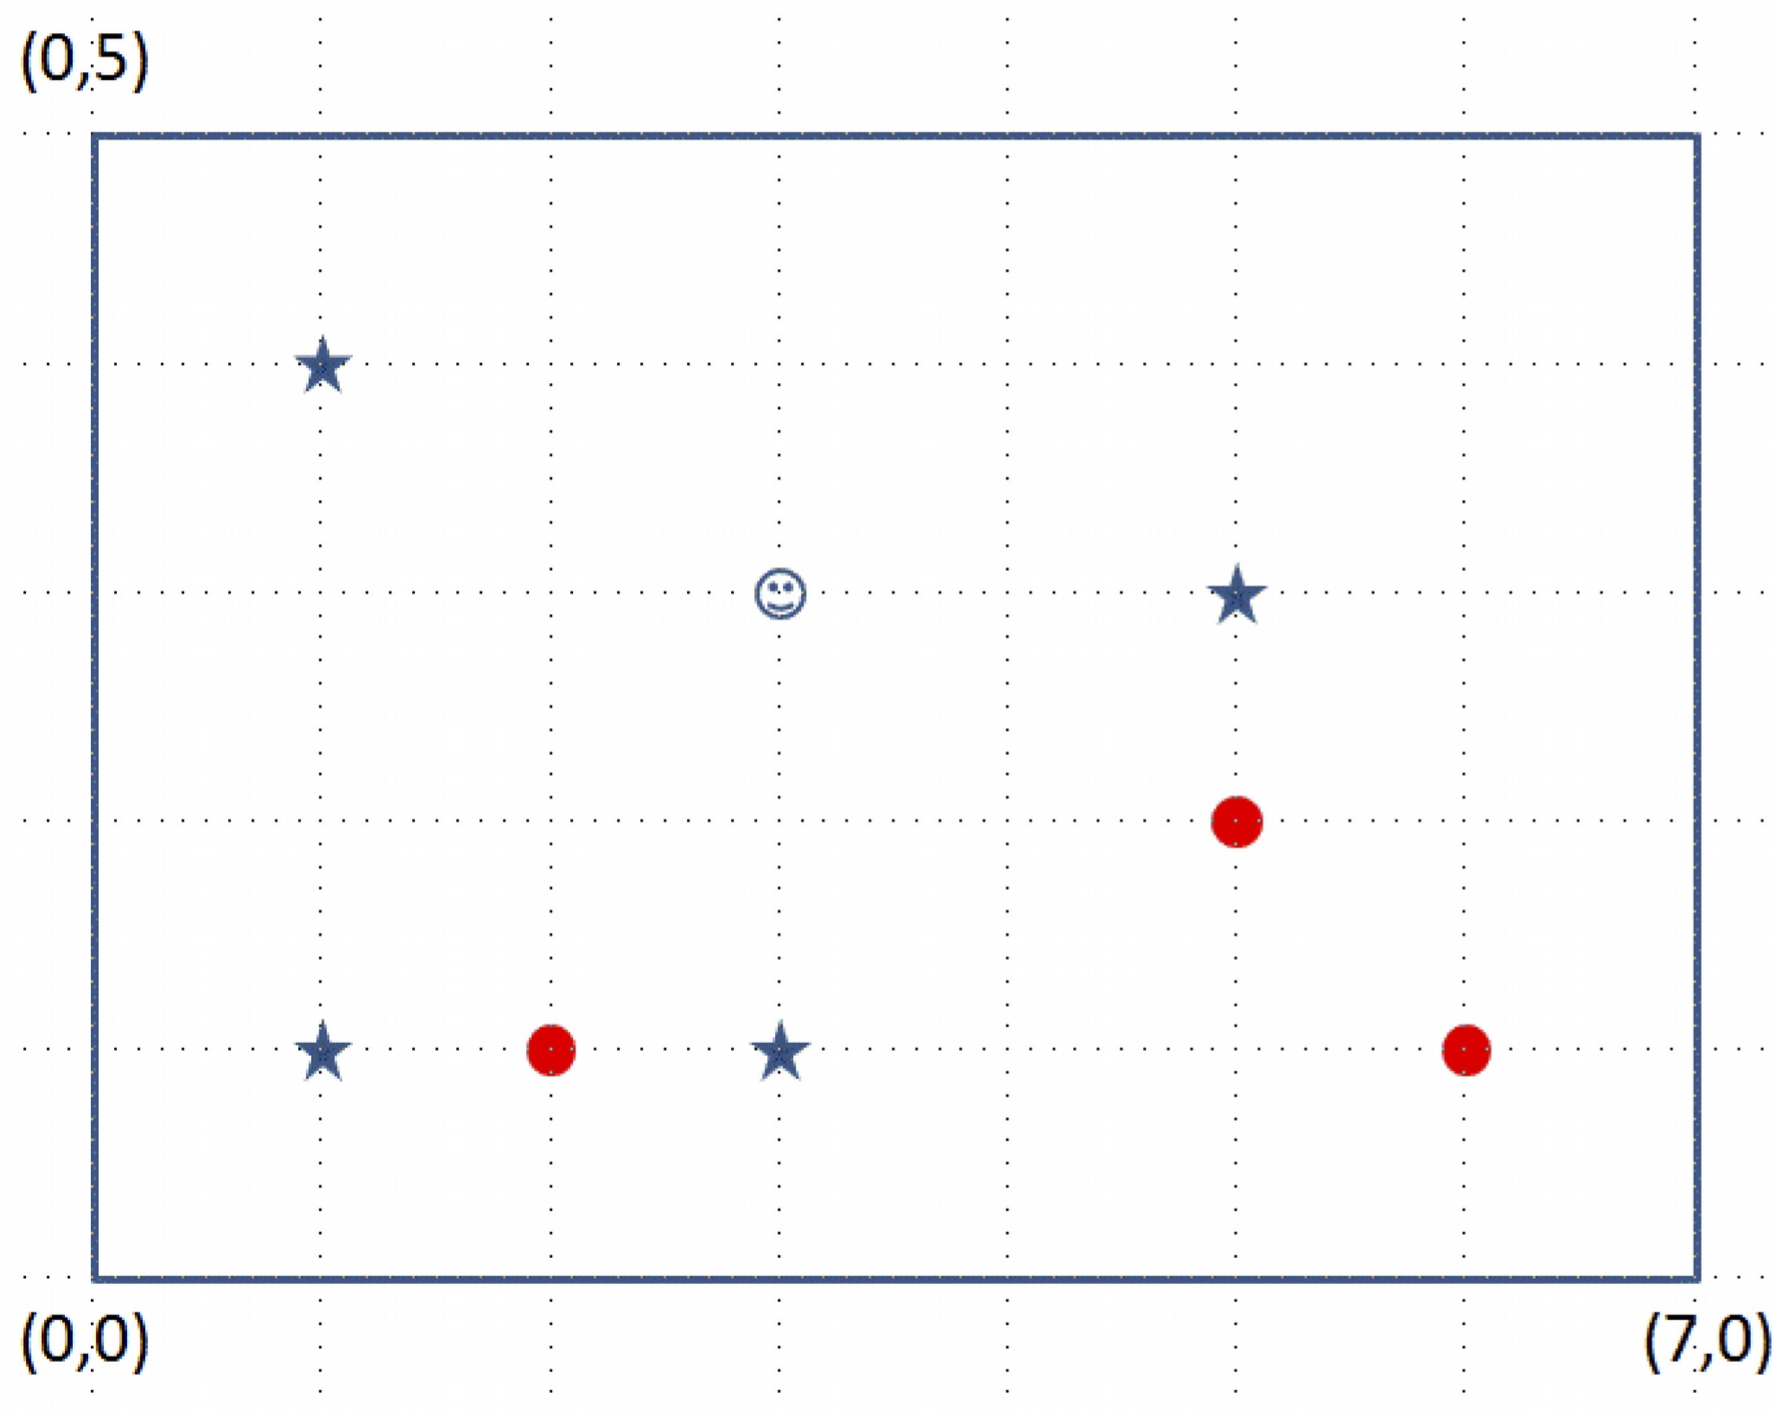
\includegraphics[width=0.5\textwidth]{exercise-1-plot}
			\end{center}
			\caption{Representación Gráfica del problema \ref{sec:e1}}
			\label{e1:plot}
		\end{figure}

		\paragraph{}
		En las ecuaciones \eqref{eq:estrellas} y \eqref{eq:circulos} se representan las instancias de cada una de las dos clases en forma de conjuntos de coordenadas. En la ecuación \eqref{eq:instancia} se muestran las coordenadas de la instancia que se desea clasificar.

		\begin{align}
		\label{eq:estrellas}
			ESTRELLAS &= \{(1,1), (1,4), (3,1), (5,3)\} \\
		\label{eq:circulos}
			CIRCULOS &= \{(2,1), (5,2), (6,1)\} \\
		\label{eq:instancia}
			instancia &= (3,3)
		\end{align}

		\paragraph{}
		Puesto que se pretende clasificar una nueva instancia apoyandose en la intuicción del algoritmo de los $k$-vecinos más cercanos, por tanto, la medida de bondad en que se basará será la distancia. Para ello se utilizará la distancia \emph{Euclídea}(\ref{sec:euclidean}), \emph{Euclídea Ponderada}(\ref{sec:euclidean_weighted}), \emph{Manhattan}(\ref{sec:manhattan}) y \emph{Hamming}(\ref{sec:hamming}).


		\paragraph{}
		Algunas de estas medidas de distancia requieren de la necesidad de normalización de los valores para poder ser calculadas de manera apropiada, por tanto el siguiente paso es normalizar los mismos respecto de cada una de las dimensiones de los datos. Para ello se ha utilizado la estrategia de normalización definida por $normalize \colon \mathbb{R}^2 \to [0,1]^2$ que se describe en la ecuación \eqref{eq:normalization}. Nótese que para ello es necesario obtener el máximo y mínimo para cada uno de los atributos, dichos resultados se muestran en las ecuaciones \eqref{eq:max_min_x} y \eqref{eq:max_min_y}.

		\begin{align}
		\label{eq:normalization}
			normalize(x,y) &= (\frac{x-min_x}{max_x-min_x},\frac{y-min_y}{max_y-min_y})
		\end{align}

		\begin{align}
		\label{eq:max_min_x}
			max_x = 6 && min_x = 1 \\
		\label{eq:max_min_y}
			max_y = 4 && min_y = 1
		\end{align}

		\paragraph{}
		Los valores normalizados se muestran en las ecuaciones \eqref{eq:estrellas_normalized}, \eqref{eq:circulos_normalized} y \eqref{eq:instancia_normalized}. Por tanto, una vez hecho esto, ya se está en condiciones de calcular las distancia de la $instancia$ a clasificar con respecto del resto de instancias y aplicar la intuición de cercanía en que se apoya el clasificador \emph{K-NN}.

		\begin{align}
		\label{eq:estrellas_normalized}
			ESTRELLAS_{normalized} &= \{(0,0), (0,1), (\tfrac{2}{5},0), (\tfrac{4}{5},\tfrac{2}{3})\} \\
		\label{eq:circulos_normalized}
			CIRCULOS_{normalized}  &= \{(\tfrac{1}{5},0), (\tfrac{4}{5},\tfrac{1}{3}), (1,0)\} \\
		\label{eq:instancia_normalized}
			instancia_{normalized}  &= (\tfrac{2}{5},\tfrac{2}{3})
		\end{align}

		\subsection{Distancia Euclídea}
		\label{sec:euclidean}

			\paragraph{}
			La \emph{Distancia Euclídea} se define tal y como se muestra en la ecuación \eqref{eq:euclidean_distance}. En este caso es necesario que los valores de entrada hayan sido normalizados previamente. Los resultados de distancia de la $instancia$ a clasificar con respecto al resto de instancias se muestran en la ecuación \eqref{eq:euclidean_distance_results}.

			\begin{align}
			\label{eq:euclidean_distance}
				D_{euclidean}(a,b) &= \sqrt{(a_x - b_x)^2 + (a_y - b_y)^2}
			\end{align}

			\begin{align}
			\label{eq:euclidean_distance_results}
				R_{euclidean} &= \{0.777_e, 0.52_e, 0.666_e, 0.4_e, 0.696_c, 0.52_c, 0.896_c\}
			\end{align}

			\paragraph{}
			El último paso es utilizar la función $min$ encargada de obtener los $k$ valores más pequeños de un determinado conjunto. Esto encaja perfectamente con lo que se pretende que haga el clasificador \emph{K-NN}. Por tanto, los valores más cercanos así como la clase en la que se clasifica $instancia$ para $k \in \{1,3,5\}$ se muestran en las ecuaciones \eqref{eq:euclidean_k_1}, \eqref{eq:euclidean_k_3} y \eqref{eq:euclidean_k_5} respectivamente.

			\begin{align}
			\label{eq:euclidean_k_1}
				min(R_{euclidean},1) &= \{ 0.4_e \} \implies instancia \in ESTRELLAS \\
			\label{eq:euclidean_k_3}
				min(R_{euclidean},3) &= \{ 0.4_e, 0.52_e, 0.52_c\} \implies instancia \in ESTRELLAS \\
			\label{eq:euclidean_k_5}
				min(R_{euclidean},5) &= \{ 0.4_e, 0.52_e, 0.52_c, 0.666_e,  0.696_e \} \implies instancia \in ESTRELLAS
			\end{align}

		\subsection{Distancia Euclídea Ponderada: $w_x=0.2, w_y=0.8$}
		\label{sec:euclidean_weighted}

			\paragraph{}
			La \emph{Distancia Euclídea Ponderada} se define tal y como se muestra en la ecuación \eqref{eq:euclidean_weighted_distance}. En este caso también es necesario que los valores de entrada hayan sido normalizados previamente. Además, la importancia que tienen cada una de las dimensiones no es igual, sino que está ponderada por los valores fijados previamente en el vector $w$. Los resultados de distancia de la $instancia$ a clasificar con respecto al resto de instancias se muestran en la ecuación \eqref{eq:euclidean_weighted_distance_results}.

			\begin{align}
			\label{eq:euclidean_weighted_distance}
				D_{w_{euclidean}}(a,b) &= \sqrt{w_x(a_x - b_x)^2 + w_y(a_y - b_y)^2} = \sqrt{0.2(a_x - b_x)^2 + 0.8(a_y - b_y)^2}
			\end{align}

			\begin{align}
			\label{eq:euclidean_weighted_distance_results}
				R_{w_{euclidean}} &= \{0.622_e, 0.347_e, 0.596_e, 0.178_e, 0.602_c, 0.347_c, 0.653_c\}
			\end{align}

			\paragraph{}
			El último paso es utilizar la función $min$ encargada de obtener los $k$ valores más pequeños de un determinado conjunto. Por tanto, los valores más cercanos así como la clase en la que se clasifica $instancia$ para $k \in \{1,3,5\}$ se muestran en las ecuaciones \eqref{eq:euclidean_weighted_k_1}, \eqref{eq:euclidean_weighted_k_3} y \eqref{eq:euclidean_weighted_k_5} respectivamente.

			\begin{align}
			\label{eq:euclidean_weighted_k_1}
				min(R_{w_{euclidean}},1) &= \{ 0.178_e \}  \implies instancia \in ESTRELLAS \\
			\label{eq:euclidean_weighted_k_3}
				min(R_{w_{euclidean}},3) &= \{ 0.178_e, 0.347_e, 0.347_c,\}  \implies instancia \in ESTRELLAS \\
			\label{eq:euclidean_weighted_k_5}
				min(R_{w_{euclidean}},5) &= \{ 0.178_e, 0.347_e, 0.347_c, 0.596_e, 0.602_c\} \implies instancia \in ESTRELLAS
			\end{align}


		\subsection{Distancia de Manhattan}
		\label{sec:manhattan}

			\paragraph{}
			La \emph{Distancia de Manhattan} se define tal y como se muestra en la ecuación \eqref{eq:manhattan_distance}. Es una medida de distancia para valores enteros, por tanto, en este caso no es apropiado utilizar las instancias normalizadas. Los resultados de distancia de la $instancia$ a clasificar con respecto al resto de instancias se muestran en la ecuación \eqref{eq:manhattan_distance_results}.

			\begin{align}
			\label{eq:manhattan_distance}
				D_{manhattan}(a,b) &= |a_x - b_x| + |a_y - b_y|
			\end{align}

			\begin{align}
			\label{eq:manhattan_distance_results}
				R_{manhattan} &= \{4_e, 3_e, 2_e, 2_e, 3_c, 3_c, 5_c\}
			\end{align}

			\paragraph{}
			El último paso es utilizar la función $min$ encargada de obtener los $k$ valores más pequeños de un determinado conjunto. Por tanto, los valores más cercanos así como la clase en la que se clasifica $instancia$ para $k \in \{1,3,5\}$ se muestran en las ecuaciones \eqref{eq:manhattan_k_1}, \eqref{eq:manhattan_k_3} y \eqref{eq:manhattan_k_5} respectivamente.

			\begin{align}
			\label{eq:manhattan_k_1}
				min(R_{manhattan},1) &= \{ 2_e \}  \implies instancia \in ESTRELLAS \\
			\label{eq:manhattan_k_3}
				min(R_{manhattan},3) &= \{ 2_e, 2_e, 3_e\}  \implies instancia \in ESTRELLAS \\
			\label{eq:manhattan_k_5}
				min(R_{manhattan},5) &= \{ 2_e, 2_e, 3_e, 3_c, 3_c, \} \implies instancia \in ESTRELLAS
			\end{align}

		\subsection{Distancia de Hamming}
		\label{sec:hamming}

			\paragraph{}
			La \emph{Distancia de Hamming} se define tal y como se muestra en la ecuación \eqref{eq:hamming_distance}. Es una medida de distancia para valores discretos, a pesar de ello, en este caso la utilizaremos con valores numéricos enteros presuponiendo que cada valor es una categoría diferente. Los resultados de distancia de la $instancia$ a clasificar con respecto al resto de instancias se muestran en la ecuación \eqref{eq:hamming_distance_results}.


			\begin{align}
			\label{eq:hamming_distance}
				D_{hamming}(a,b) &= (a_x \neq b_x) + (a_y \neq b_y)
			\end{align}

			\begin{align}
			\label{eq:hamming_distance_results}
				R_{hamming} &= \{2_e, 2_e, 1_e, 1_e, 2_c, 2_c, 2_c\}
			\end{align}

			\paragraph{}
			El último paso es utilizar la función $min$ encargada de obtener los $k$ valores más pequeños de un determinado conjunto. Por tanto, los valores más cercanos así como la clase en la que se clasifica $instancia$ para $k \in \{1,3,5\}$ se muestran en las ecuaciones \eqref{eq:hamming_k_1}, \eqref{eq:hamming_k_3} y \eqref{eq:hamming_k_5} respectivamente.

			\begin{align}
			\label{eq:hamming_k_1}
				min(R_{hamming},1) &= \{ 1_e \}  \implies instancia \in ESTRELLAS \\
			\label{eq:hamming_k_3}
				min(R_{hamming},3) &= \{ 1_e, 1_e, 2_e\}  \implies instancia \in ESTRELLAS \\
			\label{eq:hamming_k_5}
				min(R_{hamming},5) &= \{ 1_e, 1_e, 2_e, 3_c, 3_c, \}  \implies instancia \in ESTRELLAS
			\end{align}

	\section{Dígitos manuscritos}

		\paragraph{}
		[TODO]

		\begin{table}
			\centering
			\small
			\begin{tabu}{ | c | c | c | c | c | c | c | c | c | c | }
				\hline
				\multicolumn{10}{ | c | }{Validación cruzada de 10 particiones --- $K$-Vecinos más Próximos} \\ \hline
				\multirow{2}{*}{Datos}	& \multicolumn{9}{ c |}{Tasa de Error ($K=$)} \\ \cline{2-10}
																& \emph{1} & \emph{2} & \emph{3} & \emph{4} & \emph{5} & \emph{6} & \emph{7} & \emph{8}	& \emph{9}\\ \hline
				Entrenae						& $3.448\%$	 & $3.524\%$ & $3.065\%$ & $3.141\%$	& $3.371\%$ & $3.218\%$	 & $3.295\%$ & $3.295\%$ & $3.371\%$	\\
				\hline
			\end{tabu}
			\caption{Tasa de error obtenida tras realizar un experimento de Validación cruzada de 10 particiones con el clasificador \emph{K-NN} para $k \in \{1,2,...,9\}$}
			\label{table:e2}
		\end{table}



		\begin{figure}
			\begin{center}
				\begin{tikzpicture}
					\begin{axis}[
						% only scale the axis, not the axis including the ticks and labels
		        scale only axis=true,
		        % set `width' and `height' to the desired values
		        width=0.9\textwidth,
		        height=0.3\textwidth,
						]
						\addplot table [x=k, y=error, col sep=comma] {data.csv};
					\end{axis}
				\end{tikzpicture}
			\end{center}
			\caption{Representación Gráfica de la tasa de error obtenida tras realizar un experimento de Validación cruzada de 10 particiones con el clasificador \emph{K-NN} para $k \in \{1,2,...,9\}$}
			\label{plot:e2}
		\end{figure}

		\paragraph{}
		[TODO]


%-----------------------------
%	Bibliographic references
%-----------------------------
	\nocite{garciparedes:machine-learning-instance-based}
	\nocite{subject:taa}
	\nocite{tool:weka}
  \bibliographystyle{alpha}
  \bibliography{bib/misc}

\end{document}
